\documentclass[a4paper,oneside,14pt, extrafontsizes]{memoir}

 \usepackage{graphicx}
\usepackage{verbatim}
\renewcommand{\familydefault}{\sfdefault}
\chapterstyle{demo2}

\title{\emph{Conceptual Modeling Language}\\Specification\\ \small{Version 1.0}}
\author{Quenio Cesar Machado dos Santos\\
\small{Universidade Federal de Santa Catarina}\thanks{
Initially developed as part of the author's Bachelor Technical Report in Computer Sciences}}
\date{July 2017}

\makeatletter
\newcommand{\verbatimfont}[1]{\renewcommand{\verbatim@font}{\ttfamily#1}}
\makeatother

\begin{document}

\begin{titlingpage}
\maketitle
\end{titlingpage}

\frontmatter

\begin{KeepFromToc}

\clearpage
\tableofcontents

\clearpage
\listoffigures

\clearpage
\listoftables 

\end{KeepFromToc}

\mainmatter

\chapter{Introduction}
This document specifies the \emph{Conceptual Modeling Language}, or CML for short.
CML enables the modeling of the information of software systems.
It focuses on modeling the structural aspects of such systems,
having less emphasis on the behavioral aspects.
Using CML,
it is possible to represent the information as understood by the system users,
while disregarding its physical organization as implemented by target languages or technologies.

In this first part of the CML specification,
the first chapter will provide an overview of the CML compiler's architecture,
and the second chapter describes the organization and notation
used in the remainder of this document.
The second part describes that structural constructs of the language
that enable conceptual modeling.
The third part focuses on the semantics of type checking.
The fourth part covers values and expressions.
The fifth part describes code generation.
The last part will cover organization and sharing of conceptual models.


\chapter{Compiler Overview}
The CML compiler has as \emph{input},
source files defined using its own conceptual language (as specified in this document),
which provides an abstract syntax similar to (but less comprehensive than) a combination of UML \cite{uml} and OCL \cite{ocl};
and, as \emph{output}, any target languages based on extensible templates,
which may be provided by the compiler's base libraries, by third-party libraries, or even by developers.

\begin{figure}
\centering
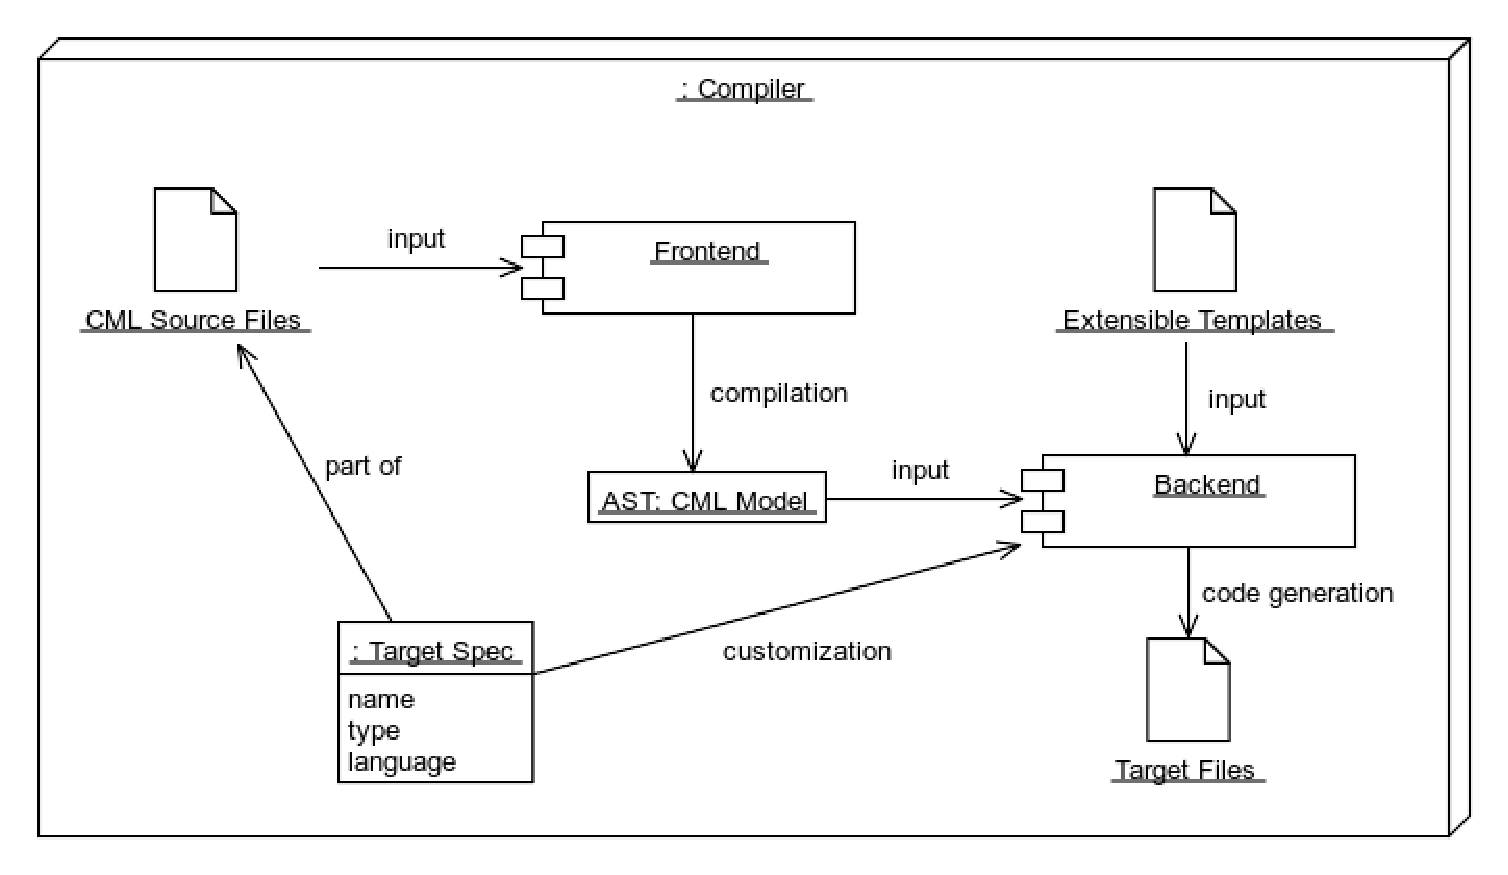
\includegraphics[width=\textwidth]{compiler/figure-overview}
\caption{An architectural overview of the CML compiler.}
\label{fig:overview}
\end{figure}

The CML compiler's overall architecture follows the standard compiler design literature \cite{torben}. An overview diagram of the architecture is shown in figure \ref{fig:overview}.
The two main components of the compiler,
and the artifacts they work with,
are presented in the next subsections.


\chapter{Concepts}
A \emph{concept} in the CML metamodel is used to represent anything
that has a coherent, cohesive meaning in a domain.
On the ER \cite{er} metamodel,
it corresponds to an \emph{entity};
on the UML \cite{uml} metamodel,
to a \emph{class}.
The CML \emph{concept} differs, however, from the UML \emph{class},
because it only contains \emph{properties},
while the UML \emph{class} may also have \emph{operations}.

Figure \ref{fig:ex:concepts} presents some examples of \emph{concepts} declared in CML.
As shown in the examples,
a \emph{concept} may have zero or more \emph{properties}
(\ref{sec:properties}),
and a \emph{property} may optionally declare a \emph{type}
(\ref{sec:primitive-types}, \ref{sec:collection-types}).
Also, as shown in the last example of figure \ref{fig:ex:concepts},
a \emph{concept} may specialize
(\ref{sec:generalization})
another \emph{concept}.

\begin{figure}
\verbatimfont{\small}
\begin{framed}
\verbatiminput{examples/concepts.cml}
\end{framed}
\caption{Concept Examples}
\label{fig:ex:concepts}
\end{figure}

Figure \ref{fig:stx:concept} specifies the syntax used
to declare a \emph{concept}.
The \textbf{concept} keyword is followed by a NAME.
Optionally, a list of other NAMEs may be enumerated,
referring to other \emph{concepts}
that are generalizations of the declared \emph{concept}.
Under the \textbf{concept} block,
a list of \emph{properties} may be declared as well.

\begin{figure}
\verbatimfont{\small}
\begin{framed}
\verbatiminput{grammar/Concepts.txt}
\end{framed}
\caption{Concept Declaration Syntax}
\label{fig:stx:concept}
\end{figure}


\chapter{Associations}
\begin{definition}
In CML,
an \emph{association} represents a relation between two \emph{concepts} (\ref{ch:concepts}),
where each \emph{concept} has an \emph{instance} in every tuple that is part of the relation.
When \emph{concepts} have an \emph{association},
its \emph{instances} are linked in such way that
it is possible to access an \emph{instance} of one \emph{concept}
from an \emph{instance} of the other \emph{concept}.
The UML \cite{uml} metamodel has a metaclass named \emph{Association} that has \emph{Property} instances,
whose \emph{types} are the \emph{Class} instances that are part of the \emph{association}.
In UML, the name of each \emph{Property} instance in the \emph{Association} metaclass
is known as the \emph{role} of the corresponding \emph{Class} in the \emph{association}.
On the CML metamodel, on other hand,
the \emph{Association} metaclass is only needed
when it is necessary to define \emph{bidirectional associations}.
For \emph{unidirectional associations},
only a \emph{property} is defined in the source \emph{concept},
making its \emph{type} the target \emph{concept}.
On the ER \cite{er} metamodel,
each \emph{association} is known as a \emph{relationship set},
and each tuple in this set is called a \emph{relationship}.
Unlike CML and UML,
the tuples in a \emph{relationship set} of an ER model
can be queried directly,
and no notion of \emph{property} is required as part of the \emph{entity type}
in order to access those \emph{relationships}.
As it is case for \emph{attributes} (\ref{ch:attributes}),
\emph{associations} in CML can also be derived from other \emph{associations}
(just as well as in UML);
they are called \emph{derived associations} (\ref{sec:derived-associations}).
\end{definition}

\begin{examples}
Figure \ref{fig:ex:associations} presents some examples of \emph{associations} declared in CML.
The concept \textbf{Vehicle} contains the property \textbf{driver},
which may optionally refer to an instance of \textbf{Employee},
meaning that a \textbf{driver} may or may not be assigned to a single \textbf{Vehicle}.
The concept \textbf{Vehicle} also has the property \textbf{owner},
which always refers to an instance of \textbf{Organization},
meaning that an \textbf{owner} must always be assigned to each instance of \textbf{Vehicle}. 
Similarly,
the concept \textbf{Employee} has the property \textbf{employer},
which must always be assigned to instance of \textbf{Organization}.
Just below the declaration of \textbf{Organization},
we observe an association named \textbf{Employment},
which enumerates two \emph{properties}:
the first is \textbf{employer} from the concept \textbf{Employee};
the second is \textbf{employees} from the concept \textbf{Organization}.
What this \emph{association} implies is a correspondence between these two properties.
Every time a reference to an instance of \textbf{Organization} is assigned to
the slot \textbf{employer} of an instance of \textbf{Employee},
a reference to this same instance of \textbf{Employee} must be assigned to
the slot \textbf{employees} of the \textbf{Organization} instance.
However,
since the \emph{type} of \textbf{employees}
in the concept \textbf{Organization}
is a sequence of \textbf{Employee} instances,
the reference to the instance of \textbf{Employee} will actually be added to the sequence,
along with the other instances already found in the sequence.
Thus, the association \textbf{Employment} actually characterizes a \emph{bidirectional association}.
The association \textbf{VehicleOwnership} is another example of a \emph{bidirectional association};
in this case,
between \textbf{Vehicle}'s \textbf{owner} property and \textbf{Organization}'s \textbf{fleet} property.
It can be noticed, though, 
in this second \emph{bidirectional association},
that the \emph{types} of the \emph{properties} are declared along with their names;
such a \emph{type} declaration,
in the \emph{association} declaration,
is optional in CML,
but must match the original \emph{property} declaration under the \emph{concept} declaration,
if present.
The \textbf{driver} property in the concept \textbf{Vehicle} is a different case,
since this \emph{property} does not participate in any \emph{association} declaration
in figure \ref{fig:ex:associations}.
That's because there is no corresponding \emph{property} in the concept \textbf{Employee}
representing the other end of the \emph{association}.
As such, the property \textbf{driver} is representing the source end of a \emph{unidirectional association}.
The property \textbf{drivers} in the concept \textbf{Organization} will be explained
in the section \ref{sec:derived-associations}.
\end{examples}

\begin{figure}
\verbatimfont{\small}
\lstinputlisting[language=cml]{examples/associations.cml}
\caption{Association Examples}
\label{fig:ex:associations}
\end{figure}


\chapter{Values}
\section{Literals}\label{sec:literals}

\begin{figure}
\verbatimfont{\small}
\begin{framed}
\verbatiminput{grammar/Literals.txt}
\end{framed}
\caption{Literals Lexical Structure}
\label{fig:literals-syntax}
\end{figure}

\section{Primitive Types}\label{sec:primitive-types}


\chapter{Expressions}

\chapter{Targets}

\chapter{Modules and Libraries}

\appendix

\chapter{Concrete Syntax (Grammar)}
\clearpage
\section{ANTLR Grammar}

\begin{framed}
\verbatimfont{\small}
\begin{verbatim}
// Compilation Units:
\end{verbatim}
\verbatiminput{grammar/CompilationUnits.txt}
\begin{verbatim}
// Concept Declarations:
\end{verbatim}
\verbatiminput{grammar/Concepts.txt}
\begin{verbatim}
// Property Declarations:
\end{verbatim}
\verbatiminput{grammar/Properties.txt}
\begin{verbatim}
// Type Declarations:
\end{verbatim}
\verbatiminput{grammar/Types.txt}
\begin{verbatim}
// Target Declarations:
\end{verbatim}
\verbatiminput{grammar/Targets.txt}
\begin{verbatim}
// Names:
\end{verbatim}
\verbatiminput{grammar/Names.txt}
\begin{verbatim}
// Literals:
\end{verbatim}
\verbatiminput{grammar/Literals.txt}
\verbatiminput{grammar/Ignored.txt}
\end{framed}


\chapter{Abstract Syntax (Metamodel)}
\input{metamodel.tex}

\chapter{Abstract Syntax Tree (Instantiation)}
\input{ast.tex}

\backmatter

\end{document}